\documentclass{standalone}

\usepackage{tikz}

\usetikzlibrary{positioning}
\usetikzlibrary{backgrounds}

\definecolor{red}{HTML}{8A3F3A}
\definecolor{yellow}{HTML}{E0BB3C}
\definecolor{blue}{HTML}{4569E0}
\definecolor{green}{HTML}{17E561}
\definecolor{other}{HTML}{6A939E}

% DTU Colors
\definecolor{dtu-corporate-red}{HTML}{990000}
\definecolor{dtu-white}{HTML}{ffffff}
\definecolor{dtu-black}{HTML}{000000}
\definecolor{dtu-blue}{HTML}{2F3EEA}
\definecolor{dtu-bright-green}{HTML}{1FD082}
\definecolor{dtu-navy-blue}{HTML}{030F4F}
\definecolor{dtu-yellow}{HTML}{F6D04D}
\definecolor{dtu-orange}{HTML}{FC7634}
\definecolor{dtu-pink}{HTML}{F7BBB1}
\definecolor{dtu-grey}{HTML}{DADADA}
\definecolor{dtu-red}{HTML}{E83F48}
\definecolor{dtu-green}{HTML}{008835}
\definecolor{dtu-purple}{HTML}{79238E}

\begin{document}

	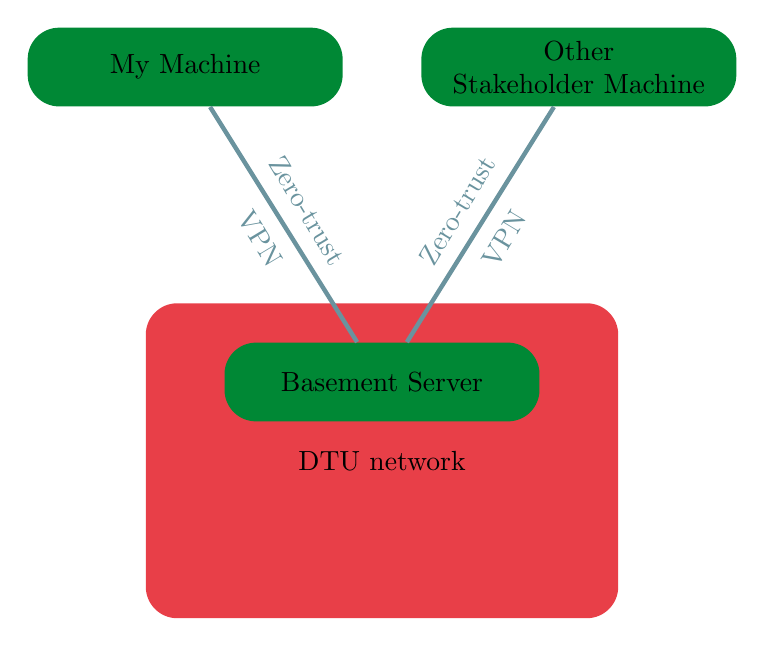
\begin{tikzpicture}

    \draw (0.0,1.0) 
		node[minimum height=4cm,fill=dtu-red,minimum width=6cm,rounded corners=0.4cm] 
			(DTU network) {DTU network};

    \draw (0.0,2.0) 
		node[minimum height=1cm,fill=dtu-green,minimum width=4cm,rounded corners=0.4cm, yshift=0cm] 
			(Basement Server) {Basement Server};

    \draw (-2.5,6.0) 
		node[minimum height=1cm,fill=dtu-green,minimum width=4cm,rounded corners=0.4cm] 
			(My Machine) {My Machine};

    \draw (2.5,6.0) 
		node[minimum height=1cm,fill=dtu-green,minimum width=4cm,rounded corners=0.4cm, align=center] 
			(Other Stakeholder Machine) {Other\\Stakeholder Machine};

	\draw[color=other,-, ultra thick] (My Machine) -- (Basement Server) 
		node[midway, above, rotate=301, fill=none, inner sep=0.2cm] {Zero-trust}
		node[midway, below, rotate=301, fill=none, inner sep=0.2cm] {VPN};

	\draw[color=other,-, ultra thick] (Other Stakeholder Machine) -- (Basement Server) 
		node[midway, above, rotate=59, fill=none, inner sep=0.2cm] {Zero-trust}
		node[midway, below, rotate=59, fill=none, inner sep=0.2cm] {VPN};

	
	\end{tikzpicture}
\end{document}
